%%%%%%%%%%%%%%%%%%%%%%%%%%%%%%%%%%%%%%%%%
% University Assignment Title Page
% LaTeX Template
% Version 1.0 (27/12/12)
%
% This template has been downloaded from:
% http://www.LaTeXTemplates.com
%
% Original author:
% WikiBooks (http://en.wikibooks.org/wiki/LaTeX/Title_Creation)
%
% License:
% CC BY-NC-SA 3.0 (http://creativecommons.org/licenses/by-nc-sa/3.0/)
%
% Instructions for using this template:
% This title page is capable of being compiled as is. This is not useful for
% including it in another document. To do this, you have two options:
%
% 1) Copy/paste everything between \begin{document} and \end{document}
% starting at \begin{titlepage} and paste this into another LaTeX file where you
% want your title page.
% OR
% 2) Remove everything outside the \begin{titlepage} and \end{titlepage} and
% move this file to the same directory as the LaTeX file you wish to add it to.
% Then add \input{./title_page_1.tex} to your LaTeX file where you want your
% title page.
%
%%%%%%%%%%%%%%%%%%%%%%%%%%%%%%%%%%%%%%%%%
%\title{Title page with logo}
%----------------------------------------------------------------------------------------
%	PACKAGES AND OTHER DOCUMENT CONFIGURATIONS
%----------------------------------------------------------------------------------------

\documentclass[12pt]{article}
\usepackage[ngerman]{babel}
\usepackage[utf8x]{inputenc}
\usepackage{amsmath}
\usepackage{nccmath}%for tiny matrices
\usepackage{graphicx}
\usepackage{grffile}%For .s in graphics
\usepackage{todonotes}%self explanatory
\usepackage{placeins}%für FloatBarriers
\usepackage[ngerman]{cleveref}%Für bessere References
\usepackage[colorinlistoftodos]{todonotes}
\usepackage{subcaption}%Für subfigures

\setlength\parindent{0pt} %Noindent for the whole document

\begin{document}

\begin{titlepage}

\newcommand{\HRule}{\rule{\linewidth}{0.5mm}} % Defines a new command for the horizontal lines, change thickness here

\center % Center everything on the page

%----------------------------------------------------------------------------------------
%	HEADING SECTIONS
%----------------------------------------------------------------------------------------

\textsc{\LARGE Georg-August-Universität Göttingen}\\[1.5cm] % Name of your university/college
\textsc{\Large }\\[0.5cm] % Major heading such as course name
\textsc{\large Numerische Strömungsmechanik}\\[0.5cm] % Minor heading such as course title

%----------------------------------------------------------------------------------------
%	TITLE SECTION
%----------------------------------------------------------------------------------------

\HRule \\[0.4cm]
{ \Large \bfseries Simulation mit FTCS- und BTCS-Verfahren}\\[0.4cm] % Title of your document
\HRule \\[1.5cm]

%----------------------------------------------------------------------------------------
%	AUTHOR SECTION
%----------------------------------------------------------------------------------------

\begin{minipage}{0.4\textwidth}
\begin{flushleft} \large
\emph{Author:}\\
Philip \textsc{Marszal} % Your name
\end{flushleft}
\end{minipage}
~
\begin{minipage}{0.4\textwidth}
\begin{flushright} \large
\emph{Prüfer:} \\
Prof. Dr. Andreas \textsc{Tilgner} % Supervisor's Name
\end{flushright}
\end{minipage}\\[2cm]

% If you don't want a supervisor, uncomment the two lines below and remove the section above
%\Large \emph{Author:}\\
%John \textsc{Smith}\\[3cm] % Your name

%----------------------------------------------------------------------------------------
%	DATE SECTION
%----------------------------------------------------------------------------------------

{\large \today}\\[2cm] % Date, change the \today to a set date if you want to be precise

%----------------------------------------------------------------------------------------
%	LOGO SECTION
%----------------------------------------------------------------------------------------


\includegraphics{logo_1.jpg}\\[1cm] % Include a department/university logo - this will require the graphicx package

%----------------------------------------------------------------------------------------

\vfill % Fill the rest of the page with whitespace

\end{titlepage}


\begin{abstract}
Im Zuge dieses Projektes wird das Verhalten der BTCS und FTCS am Beispiel der Integration der Konvektions-Diffusions-Gleichung behandelt. Es wurden zwei C++ Anwendungen zu Integration der Gleichung erstellt, die benutzt wurden um Fehler, Stabilität und Laufzeit der beiden Verfahren zu untersuchen. Der Fehler des FTCS Verfahren nimmt mit feinerer Aufteilung des Gitters ab, führt aber bei gleichbleibender Zeitdiskretisierung bei hohen Peclet-Zahlen zu Instabilität. Die numerische Suche nach der Instabilitätsgrenze stößt bei begrenzten Integrationszeiträumen an ihre Grenze.

Für das in der BTCS-Methode verwendete SOR-Verfahren wurden optimale Werte des Relaxationsparameters bestimmt. Für einen Zeitschritt von 100 und einer Peclet-Zahl von 10, wurde dieser bei einem Wert von etwa 1.7 gefunden.

Der Vergleich zwischen BTCS und FTCS ergibt wenig Abweichung in Genauigkeit. Das BTCS-Verfahren ist jedoch mit einem größeren Programmieraufwand verbunden und braucht zur Integration des gleichen Zeitraums, bei kleinen Zeiten, ca. 60 mal so viel Zeit.
\end{abstract}

\section{Einleitung}
Obwohl die Navier-Stokes-Gleichungen seit der ersten Hälfte des 19ten Jahrhunderts bekannt sind, gibt es heute noch immer keine allgemeine analytische Lösung dieser.
Die Hartnäckigkeit dieses Problem hat das \emph{Clay Mathematics Institute} sogar dazu gebracht ein 1 Millionen \$ Ausschreiben auf die Lösung der Gleichungen auszusetzen.

Für die Untersuchung strömungsdynamischer Systeme, ist man daher nahezu vollkommen auf numerische Methoden angewiesen.

Ein Beispiel für die Integration der Konvektions-Diffusions-Gleichung wird hier mit den beiden finiten Differenzenmethoden FTCS und BTCS
diskutiert.

\newpage
\section{Problemstellung}
In diesem Projekt geht es um die Untersuchung der Konvektions-Diffusions-Gleichung(KDG) mit einem unterliegenden Geschwindigkeitsfeld.
Interpretieren lässt sich diese zum Beispiel als ein Temperaturfeld in einem Fluid als Medium.
Die zeitliche Veränderung dieses Feldes wird dann durch zwei verschiedene Wärmetransportarten verursacht.
Zum einen breitet sich die Temperatur durch Diffusion (Brownsche-Teilchenbewegung) aus. In der KDG tritt diese Ausbreitungart als zweite Ableitung im Ort auf.

Die zweite Transportart, die in einem Fluid auftritt, ist die Konvektion. Wärme wird die sich bewegende Flüssigkeit transportiert. Dies entspricht einem Skalarprodukt von Gradientem mit dem Geschwindigkeitsfeld in der KDG.

\cref{Gl:PDGL} ist die entdimensionalisierte Form der KDG.
\begin{align}
  \frac{\partial T(\boldsymbol x, t)}{\partial t} + \text{Pe}~ \boldsymbol{u}_0\cdot \nabla T(\boldsymbol x, t) = \nabla^2 T(\boldsymbol x, t). \label{Gl:PDGL}
\end{align}

Das konkrete Problem wird durch die Randbedingungen und das Geschwindigkeitsfeld charakterisiert.
Das System ist zunächst auf eine quadratische Box, $0\leq x \leq 1$ und $0\leq y \leq 1$, eingeschränkt.
An den Rändern der Box werden folgende Randbedingungen angenommen:
\begin{align}
  \begin{split}
  T(t,x,y=0) = 0, &  T(t,x,y=1)=1, \\
  \left.\frac{\partial T}{\partial x}\right|_{x=0} =& \left.\frac{\partial T}{\partial x}\right|_{x=1} = 0.
\end{split}
\end{align}

Das Geschwindigkeitsfeld ist durch \cref{eq:uv} gegeben.
\begin{align}
  \boldsymbol u(x,y) =
  \begin{pmatrix}
    u(x,y)\\
    v(x,y)
  \end{pmatrix} =
  \begin{pmatrix}
    \pi \sin{2\pi x}\cos{\pi y}\\
    -2\pi \cos{2\pi x}\sin{\pi y}
  \end{pmatrix}\label{eq:uv}
\end{align}
Eine kurze Rechnung ergibt, dass das Feld divergenzfrei ist. \cref{fig:uv} zeigt das Geschwindigkeitsfeld in der Box.
\begin{figure}
  \centering
  \begin{subfigure}[b]{0.45\textwidth}
  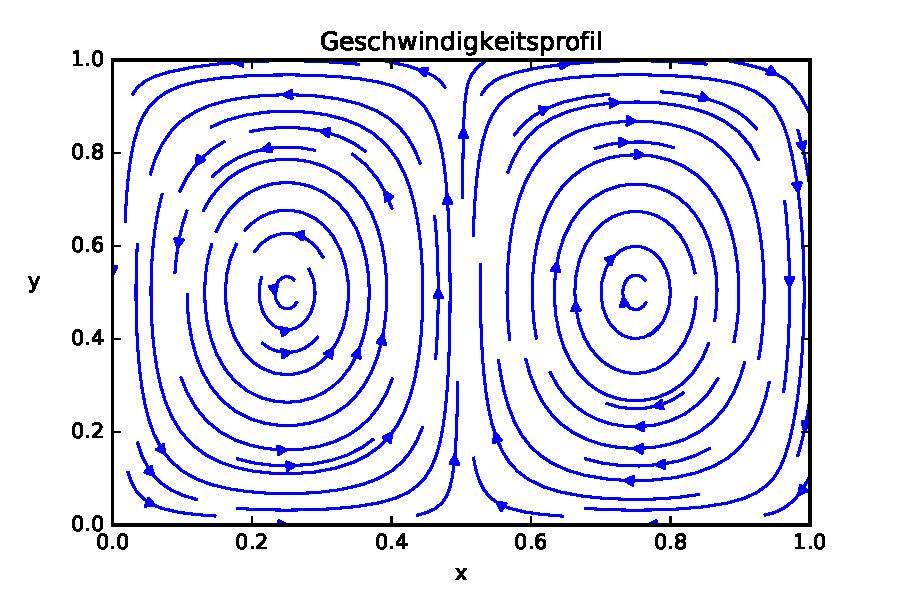
\includegraphics[width=\textwidth]{/home/marszal/Projects/Num_Str_final/Protokoll/geschw.pdf}\caption{\centering Geschwindigkeitsfeld \\ in der Box.}\label{fig:uv}
  \end{subfigure}
  ~
  \begin{subfigure}[b]{0.45\textwidth}
  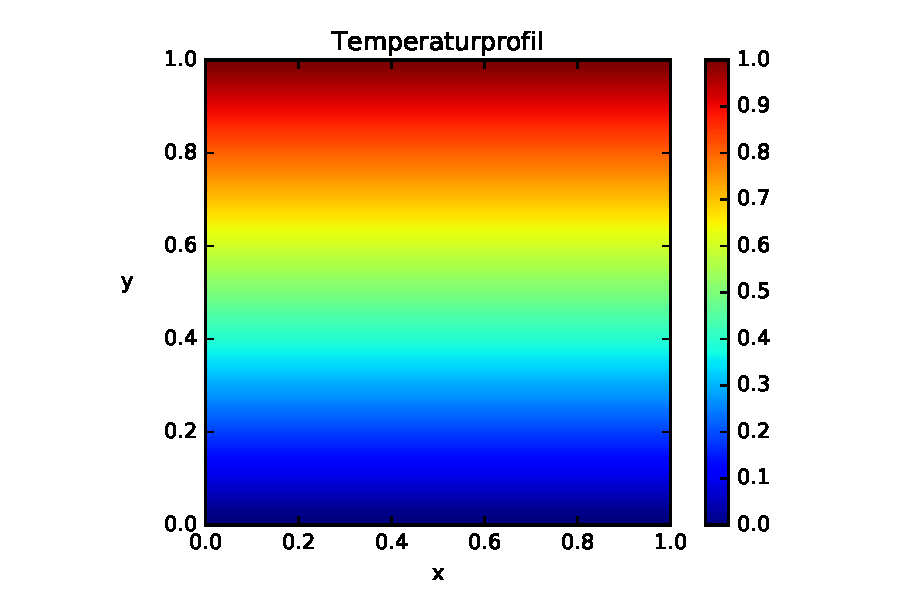
\includegraphics[width=\textwidth]{/home/marszal/Projects/Num_Str_final/Protokoll/T0.pdf}\caption{\centering Temperaturverteilung zur Zeit $t=0$.}\label{fig:t0}
  \end{subfigure}
  \caption{Geschwindigkeitsfeld und Anfangsbedingung des Systems}
\end{figure}

Die Anfangsbedingung an das Temperaturfeld lautet
\begin{align}
  T(0,x,y) = y \nonumber
\end{align}
und ist in \cref{fig:t0} dargestellt.

Zur Überprüfung der hier erstellten Verfahren ist es notwendig eine Referenzlösung zur Verfügung zu haben.
Dazu gibt es die Möglichkeit eine inhomogene Temperaturverteilung zu wählen und die KDG mittels eines Quellterms $Q$ so anzupassen, dass die gewählte Lösung eine stationäre Lösung der modifizierten Gleichung ist.

Als Wunschlösung wird das Temperaturfeld $T^* = \cos{\pi x}\sin{\pi y}+y$ gewählt. Die neue Differentialgleichung des Problems
lautet nun:
\begin{align}
  \frac{\partial T(\boldsymbol x, t)}{\partial t} + \text{Pe}~ \boldsymbol{u}_0\cdot \nabla T(\boldsymbol x, t) = \nabla^2 T(\boldsymbol x, t) + Q(x,y). \label{Gl:PDGL_Quell}
\end{align}
Durch Einsetzen von $T^*$ in diese Gleichung lässt sich der Quellterm $Q$ bestimmen als \cref{eq:quelle}
\begin{align}
  \begin{split}
  Q = &- Pe~ \pi^2 \sin{2 \pi x} \cos{\pi y} \sin{\pi x} \sin{\pi y} \\
   &- 2 Pe~ \pi^2 \cos{2 \pi x} \cos{\pi y} \cos{\pi x} \sin{\pi y}\\
   &- 2 Pe~ \pi \cos{2 \pi x} \sin{\pi y}\\
   &+ 2 \pi^2 \cos{\pi x} \sin{\pi y}.
 \end{split}\label{eq:quelle}
\end{align}
\cref{fig:qtstat} zeigt die stationäre Lösung $T^*$ und die Quelle $Q$.
\begin{figure}
  \centering
  \begin{subfigure}[b]{0.45\textwidth}
  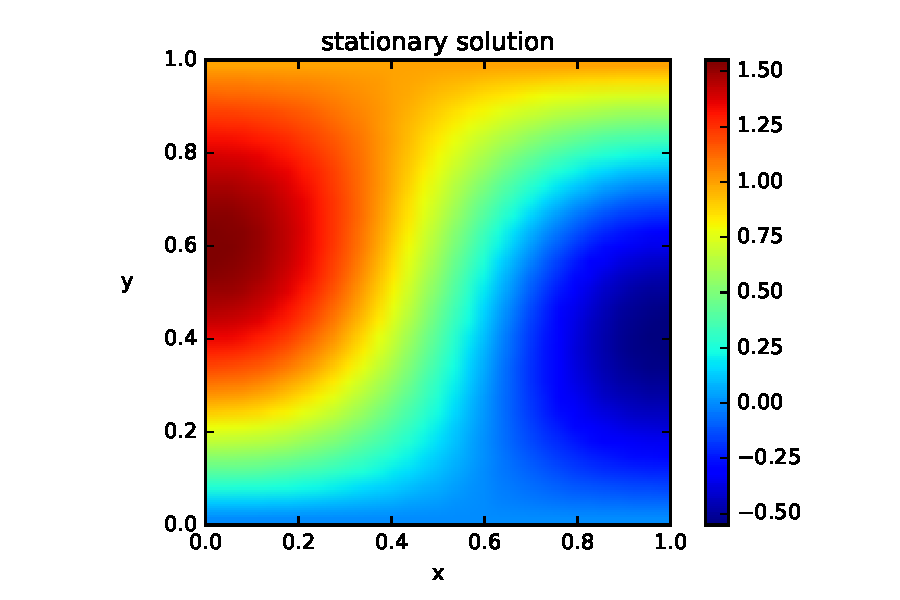
\includegraphics[width=\textwidth]{/home/marszal/Projects/Num_Str_final/Protokoll/Tstat.pdf}\caption{\centering Stationäre Lösung $T^*$}
  \end{subfigure}
  ~
  \begin{subfigure}[b]{0.45\textwidth}
  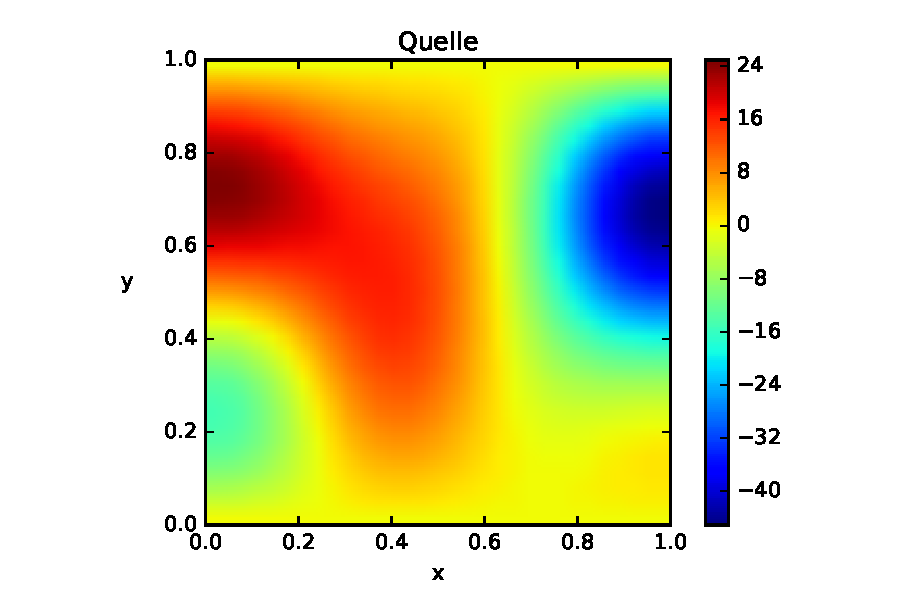
\includegraphics[width=\textwidth]{/home/marszal/Projects/Num_Str_final/Protokoll/Quelle.pdf}\caption{Quellterm $Q$}
\end{subfigure}\caption{Stationäre Lösung $T^*$ und Quellterm $Q$ aus \cref{Gl:PDGL_Quell}.}
  \label{fig:qtstat}
\end{figure}

\newpage
\section{Methoden}
Zur Simulation von Strömungsmechanikproblemen kommen eine Vielzahl verschiedener Verfahren in Frage.
Ein konzeptionell simples Verfahren, das häufig Anwendung findet, ist die \emph{Finite-Differenzen-Methode}.
Diese wird zum Lösen des hier gestellten Problems verwendet.
Andere Verfahren die zur Lösung dieser Art von Problem eingesetzt werden können sind \emph{Finite-Volumen-Methoden}, \emph{Finite-Elemente-Verfahren} und \emph{spektrale Verfahren}.
Bei fast allen Verfahren liegt die Diskretisierung des integrierten Systems durch ein Gitter zu Grunde, welches die theoretisch kontinuierliche Lösungsfunktion approximiert.
\subsection{Finite-Differenzen-Verfahren}
Um eine partielle Differentialgleichung numerisch zu integrieren, müssen die Ableitungen ersetzt werden durch diskret berechenbare Terme.
Ein naiver Ansatz ist die Näherung der Ableitung $T'(x)$ einer Funktion an einem Punkt durch den Differenzenquotienten.
\begin{align}
  T'(x) = \lim_{h\rightarrow 0}\frac{T(x+h)-T(x)}{h}.\label{Gl:dq1O}
\end{align}
Bei der Verwendung eines Gitters entspricht hier $h$ dem Abstand der zwei benachbarten Gitterpunkte.
Der Differenzenquotient in \cref{Gl:dq1O} entspricht dem Vorwärtsdifferenzenquotienten erster Ordnung in $h$.

Eine Approximation höherer Ordnung erhält man z.B. durch den zentralen Differenzenquotienten
\begin{align}
  T'(x) = \frac{T(x+h)-T(x-h)}{2h} + O(h^2),\label{Gl:dq2O}
\end{align}
oder für die zweite Ableitung als Vorwärtsdifferenzenquotient von $T'(x)$:
\begin{align}
  T''(x) = \frac{T(x+h)-2T(x)+T(x-h)}{h^2}+O(h^2).\label{Gl:dq2O2Abl}
\end{align}
Durch Kombinationen unterschiedlicher Differenzenquotienten können Näherungen höherer Ordnung erhalten werden.
\subsection{FTCS-Variante}
Verwendet man zur Diskretisierung der PDGL eine Vorwärtsdifferenz für die Zeitableitung und eine zentrale Differenz für die Ortsableitungen, so spricht man von einem \emph{FTCS}-Verfahren (\textbf{F}orwards \textbf{T}ime \textbf{C}entral \textbf{S}pace).
Diskretisiert man \cref{Gl:PDGL} auf diese Weise so erhält man die Differenzengleichung:
\begin{align}
  \begin{split}
  \frac{T^{n+1}_{i,j}-T^{n}_{i,j}}{\Delta t} + \text{Pe}~ u_{i,j} \frac{T^{n}_{i+1,j}-T^{n}_{i-1,j}}{\Delta x} + \text{Pe}~ v_{i,j} \frac{T^{n}_{i,j+1}-T^{n}_{i,j-1}}{\Delta y}\\
   =  \frac{T^{n}_{i+1,j}-2T^{n}_{i,j}+T^{n}_{i-1,j}}{\Delta x^2} +\frac{T^{n}_{i,j+1}-2T^{n}_{i,j}+T^{n}_{i,j-1}}{\Delta y^2}
 \end{split}\label{Gl:FTCS}
\end{align}
Hierbei entspricht $\Delta t$ dem Zeitschritt, $\Delta x = 1./N_x$ und $\Delta y = 1./N_y$ entsprechen den jeweiligen Gitterabständen in $x$- und $y$-Richtung.
Um den Rand des Systems zu betrachten werden $(N_x+1) \cdot (N_y+1)$ Gitterpunkte betrachtet.
\cref{Gl:FTCS} kann nun numerisch integriert werden, indem $T^{n+1}_{i,j}$ für jeden Gitterpunkt berechnet wird.
Allerdings ist darauf zu achten ob man $T^{n+1}_{i,j}$ am Rand berechnet, denn hier müssen die Randbedingungen in die Gleichung eingebaut werden.

Die Dirichlet Randbedingungen lassen sich unproblematisch für $T^{n}_{i,0}$ und $T^{n}_{i,N_y+1}$ einsetzen. Diese Gitterpunkte verändern sich nicht im Laufe der Zeit, müssen also nicht integriert werden.
Anders sieht dies allerdings für die Neumann Randbedingungen aus. Die Gitterpunkte mit $i=0$ und $i=N_x+1$ verändern sich sehr wohl im Laufe der Zeit.

Um zu vermeiden, dass man auf Gitterpunkte außerhalb des Gitters zugreift, muss man eine Vorwärtsdifferenz verwenden.
Eine Näherung zweiter Ordnung für die Ableitung $\frac{\partial T(\boldsymbol x,t)}{\partial x}$ bei $x=0$ und $x=1$ lässt sich mit \cref{Gl:forw2} berechnen:
\begin{align}
  \begin{split}
  T^{n+1}_{0,j} = -\frac{1}{3} \left( T^{n+1}_{2,j}-4T^{n+1}_{1,j}\right), \\
  T^{n+1}_{N_x+2,j} = -\frac{1}{3} \left( T^{n+1}_{N_x,j}-4T^{n+1}_{N_x+1,j}\right).
\end{split}\label{Gl:forw2}
\end{align}

Mit \cref{Gl:FTCS} und \cref{Gl:forw2} ist man nun in der Lage das das Problem zu simulieren.

\subsection{Die BTCS-Variante}
Im Gegensatz zu dem FTCS-Verfahren, welches ein explizites Verfahren zu Lösung von partiellen Differentialgleichungen darstellt, handelt es sich bei der \emph{BTCS}-Methode (\textbf{B}ackwards \textbf{T}ime \textbf{C}entral \textbf{S}pace) um ein implizites Verfahren.
Implizite Verfahren erfordern die Lösung eines Gleichungssystems ehe ein Zeitschritt durchgeführt werden kann, garantieren im Gegenzug dafür aber Kovergenz.

Im BTCS-Verfahren wird die Zeitableitung durch eine Rückwärtsdifferenz diskretisiert. Dadurch entsteht in dem vorliegenden Problem zunächst ein lineares Gleichungssystem aus $(N_x+1)\cdot (N_y+1)$ Gleichungen für die $T^n_{i,j}$.
\begin{align}
  \begin{split}
  \frac{T^{n}_{i,j}-T^{n-1}_{i,j}}{\Delta t} + \text{Pe}~ u_{i,j} \frac{T^{n}_{i+1,j}-T^{n}_{i-1,j}}{\Delta x} + \text{Pe}~ v_{i,j} \frac{T^{n}_{i,j+1}-T^{n}_{i,j-1}}{\Delta y}\\
   =  \frac{T^{n}_{i+1,j}-2T^{n}_{i,j}+T^{n}_{i-1,j}}{\Delta x^2} +\frac{T^{n}_{i,j+1}-2T^{n}_{i,j}+T^{n}_{i,j-1}}{\Delta y^2}
 \end{split}\label{Gl:BTCS}
\end{align}
Führt man die Dirichlet-Randbedingungen ein so reduziert sich das Gleichungssystem auf $N_x \cdot (N_y-1)$ Gleichungen. Um die Neumann-Randbedingungen mit dem Gleichungssystem zu vereinigen betrachtet man den zentralen Differenzenquotienten an $x=0$ und $x=1$:
\begin{align}
  \left. \frac{\partial T}{\partial x}\right|_{x=0} = \frac{T^{n}_{1,j}-T^{n}_{-1,j}}{\Delta x} = 0, \nonumber
\end{align}
und einem analogen Quotienten für $x=1$. Mithilfe dieser Gleichungen lassen sich die Terme $T^{n}_{-1,j}$ und $T^{n}_{N_x+2,j}$ aus dem Gleichungssystem eliminieren und somit die Neumann-Randbedingungen in die Gleichungen einbauen.

Um dieses System zu lösen bietet es sich an das Gitter $T^n_{i,j}$ als $N_x \cdot (N_y-1)$ dimensionalen Vektor umzuschreiben.
Die Lösung des Systems entspricht dann einer Invertierung der Matrix $M$, die sich aus den Gleichungen als \cref{Gl:Matrix} ergibt.

\begin{align}
M=\left(\begin{medsize}\begin{smallmatrix}
(1.+4D)      & (v_{0,1}A-D) & 0          & ...       & -2D       & 0        &...       &&...       &&0    \\
-(v_{0,2}A+D) & (1.+4D)      & (v_{0,2}A-D) & 0         & ...      & -2D       &0       &&...       &&0    \\
0          &-(v_{0,3}A+D)  & (1.+4D)      &(v_{0,3}A-D) &0         &...       &       & &...       &&0 \\
...          & ...        &...         &...        &...       &...       &...       &...&...       &&0\\
...          &  ...       &-(u_{i,j}A+D)  &...        &-(v_{i,j}A+D)&(1.+4D)     &(v_{i,j}A-D)& ...      & (u_{i,j}A-D)&... 0\\
    ...         & ...        &...         &...        &...       &...       &...       &...&...       &&0\\
0          &...         &            &...        &           &         &-2D          &...       &-(v_{N_x+1,N_y}A+D) &(1.+4D)
\end{smallmatrix}\end{medsize}\right)\label{Gl:Matrix}
\end{align}



Hierbei wurde der Vektor $\boldsymbol T^n$ so gewählt, dass die Spalten des Gitters aneinander gehängt werden, sprich die Komponenten des Vektors laufen zunächst im $j$-Index durch : $\boldsymbol T^n = \left( T^n_{0,1}, T^n_{0,2}, ..., T^n_{0,N_y}, T^n_{1,1},...,T^n_{N_x+1,N_y} \right)$.
Die Terme $A=\frac{Pe~\Delta t}{\Delta x}$ und $D=\frac{\Delta t}{\Delta x^2}$ enstprechen den konstanten Vorfaktoren im Advektions- und Diffusionsterm.

\newpage
\subsection{Der SOR-Algorithmus}
Die Matrix $M$ hat für vernünftige Gittergrößen und Zeitschritte $\Delta t$ die Eigenschaft, dass sie diagonal dominant ist. Also die Summe der Beträge der nicht-diagonalen Einträge in jeder Spalte nicht den Betrag des diagonalen Eintrags dieser Spalte übersteigt.

Für Matrizen mit dieser Eigenschaft liefert das sogenannte Gauß-Seidel-Verfahren eine approximative Lösung des Gleichungssystems $ M\boldsymbol x = \boldsymbol b$, die garantiert gegen die tatsächliche Lösung konvergiert.
Zunächst wird $M$ in eine Summe aus untere und oberer Dreiecksmatrix, $L$ und $U$, und der Diagonale $D$ zerlegt. Die Iterationsvorschrift des Gauß-Seidel-Verfahrens sieht nun wie folgt aus:
\begin{align}
  \boldsymbol x_{n+1} = (L+D)^{-1}(\boldsymbol b - U\boldsymbol x_{n}) \label{eq:gss}
\end{align}
Der Vorteil dieser Methode liegt darin, dass das Produkt von $(L+D)^{-1}$ mit einem Vektor einfach über Vorwärtssubstitution berechnet werden kann, dank der Dreiecksform von $L+D$.

Eine Weiterentwicklung des Gauß-Seidel-Algorithmus ist die \emph{successive overrelaxation}-Methode (SOR). Dazu wird \cref{eq:gss} zunächst durch den Korrekturvektor $\boldsymbol r_n = M\boldsymbol x_n -\boldsymbol b$ ausgedrückt.
Über den Relaxationsparameter $\omega$ kann nun die Konvergenz des Gauß-Seidel-Verfahrens erheblich beschleunigt werden.
Die Iterationsvorschrift des SOR-Algorithmus lautet:
\begin{align}
  \boldsymbol x_{n+1} = \boldsymbol x_n - \omega (L+D)^{-1}(\boldsymbol r_n) \label{eq:sor}
\end{align}
Für die Wärmetransportgleichung liegt der optimale Relaxationsparameter zwischen 0 und 2.

\newpage
\section{Programmstruktur}

\begin{figure}\centering
  %\input{FTCSflow.pdf_tex}
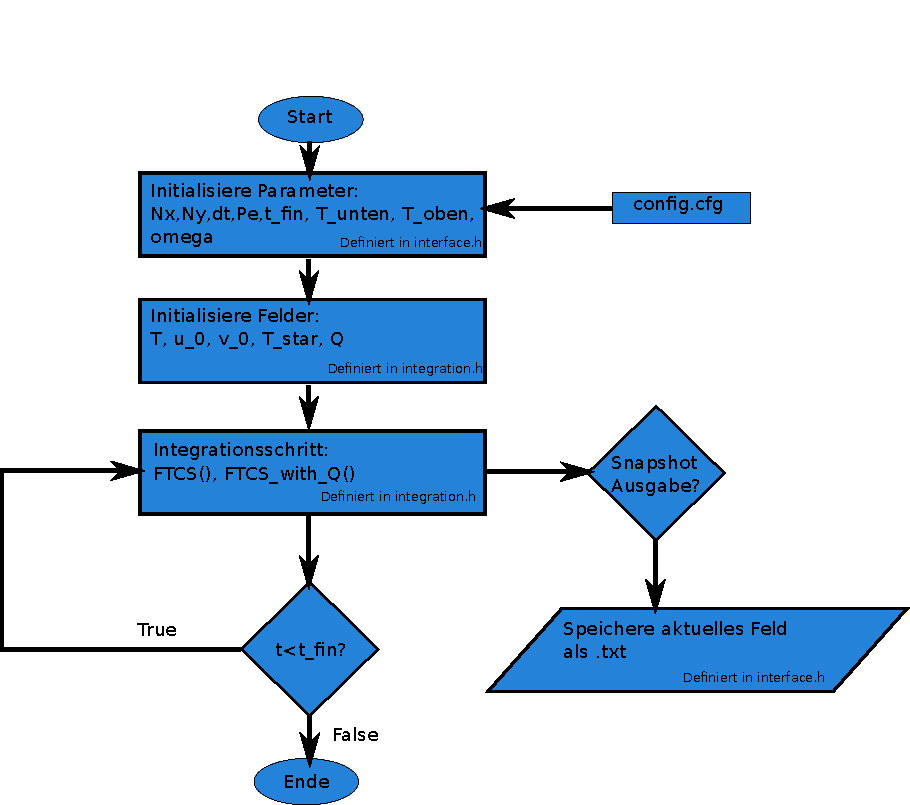
\includegraphics[height=0.45\textheight]{FTCSflow.pdf}\caption{Flowchart der Implementierung der FTCS-Methode.}\label{fig:FTCS}
\end{figure}

Zur Bearbeitung des Problems wurden die beiden Methoden, FTCS und BTCS, in zwei getrennten Programmen implementiert. Als interface mit den Programmen wurde eine Konfigurationsdatei erstellt, die es erlaubt Parameter der Algorithmen zu ändern, ohne das Programm neu komplilieren zu müssen.
Die Interaktion mit der Konfigurationsdatei wurde in der Headerdatei \emph{interface.h} implementiert, welche zudem sämtliche Funktionen zur Ausgabe der Ergebnisse beinhaltet.

Die Kernfunktionen der Integration befinden sich in der \emph{integration.h}-Datei. Diese sind die Initialisierungen der Temperaturfelder, des Quellfeldes und der Geschwindigkeitsfelder.
Außerdem sind einzelne Zeitschritte in den Funktionen \emph{FTCS()} und \emph{FTCS\_with\_Q()} zusammengefasst. Diese nehmen als Input das Temperaturfeld (call-by-reference), die Geschwindigkeitsfelder und das Quellfeld (call-by-value).
Die Entscheidung, welche Gleichung integriert werden soll, wird in der Konfigurationsdatei getroffen.
\FloatBarrier
\newpage

\begin{figure}\centering
  %\input{FTCSflow.pdf_tex}
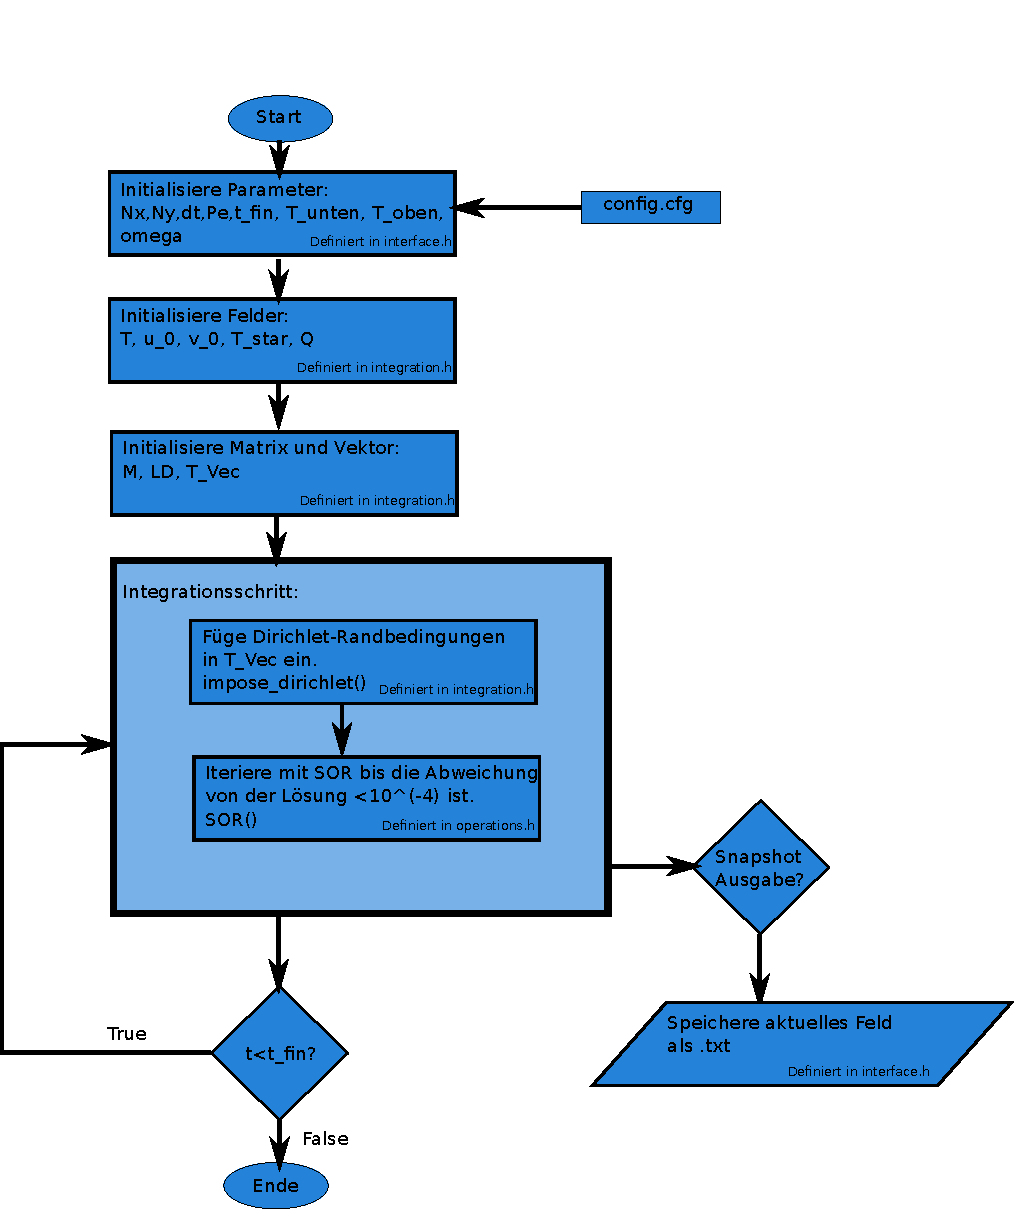
\includegraphics[height=0.45\textheight]{BTCSflow.pdf}\caption{Flowchart der Implementierung der BTCS-Methode.}\label{fig:BTCS}
\end{figure}

Die BTCS-Methode benötigt weitere Funktionen, die von dem betrachteten Problem abhängen. Dies sind Funktionen zum transformieren des Feldes in einen Vektor und zurück (\emph{reshape\_vector()} und \emph{shape\_back()}), die Einführung der Dirichlet-Randbedingungen in den Vektor (\emph{impose\_dirichlet()}) und die Initialisierung der Matrix $M$ (\emph{BCTS\_implicit\_Matrix()}).

Im BTCS Programm werden zudem algebraische Operationen benötigt, die in der Datei \emph{operations.h} definiert sind.
Dabei handelt es sich um standard Vektor-Matrix Operationen, aber auch die Triangularisierung der $M$-Matrix (\emph{triangularize()}) und das von der Problemstellung unabhängige SOR-Verfahren (\emph{SOR()}).

Innerhalb der Schleife über die Zeit wurde zudem eine Abfrage eingeführt, die zu in der Konfigurationsdatei definierten Zeitpunkten das aktuelle Temperaturfeld ausgibt.

Die Darstellung der Ergebnisse wurde mittels \emph{Python-Matplotlib} durchgeführt.


\FloatBarrier
\newpage
\section{Ergebnisse}
Die anfängliche Betrachtung des Temperaturfeldes im Verlauf der Zeit, wie es durch die FTCS-Methode berechnet wird, liefert die Ergebnisse in \cref{fig:FTCSnaive}. Hiefür wurde eine Peclet-Zahl von $Pe~=10$ und ein Gitter von $N_x=N_y=30$ angenommen. Die Schrittweite in der Zeit beträgt $dt=0.0002$.

\begin{figure}
\centering
  \begin{subfigure}[b]{0.35\textwidth}
    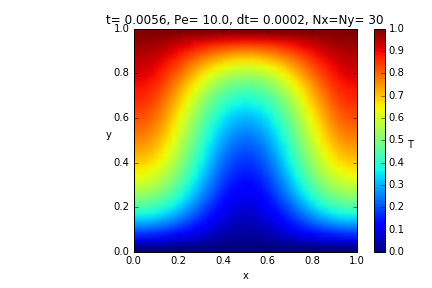
\includegraphics[width=1.15\textwidth]{/home/marszal/Projects/Num_Str_final/FTCS/plots/all/0.0056_10_30_30_0.0002_0.txt.png}
  \end{subfigure}
  ~
  \begin{subfigure}[b]{0.35\textwidth}
    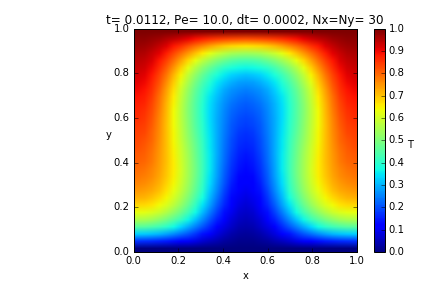
\includegraphics[width=1.15\textwidth]{/home/marszal/Projects/Num_Str_final/FTCS/plots/all/0.0112_10_30_30_0.0002_0.txt.png}
  \end{subfigure}
  \\
  \begin{subfigure}[b]{0.35\textwidth}
    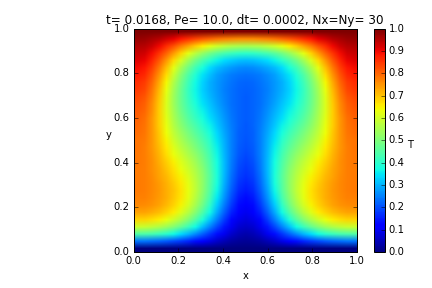
\includegraphics[width=1.15\textwidth]{/home/marszal/Projects/Num_Str_final/FTCS/plots/all/0.0168_10_30_30_0.0002_0.txt.png}
  \end{subfigure}
  ~
  \begin{subfigure}[b]{0.35\textwidth}
    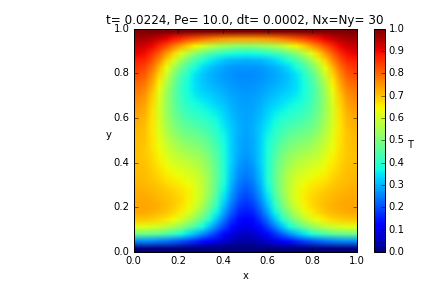
\includegraphics[width=1.15\textwidth]{/home/marszal/Projects/Num_Str_final/FTCS/plots/all/0.0224_10_30_30_0.0002_0.txt.png}
  \end{subfigure}
  \\
  \begin{subfigure}[b]{0.35\textwidth}
    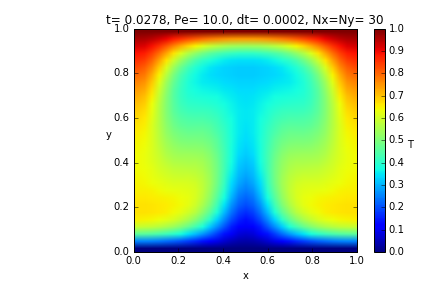
\includegraphics[width=1.15\textwidth]{/home/marszal/Projects/Num_Str_final/FTCS/plots/all/0.0278_10_30_30_0.0002_0.txt.png}
  \end{subfigure}
  ~
  \begin{subfigure}[b]{0.35\textwidth}
    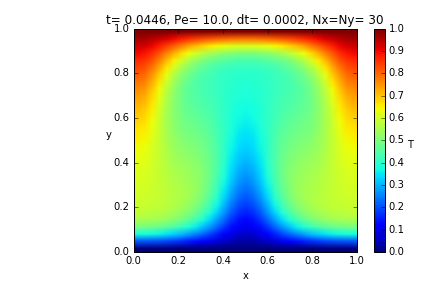
\includegraphics[width=1.15\textwidth]{/home/marszal/Projects/Num_Str_final/FTCS/plots/all/0.0446_10_30_30_0.0002_0.txt.png}
  \end{subfigure}
\caption{Temperaturfeld zu verschiedenen Zeiten. Berechnet mit dem FTCS-Verfahren.}\label{fig:FTCSnaive}
\end{figure}
\FloatBarrier
\newpage
\subsection{Fehler der FTCS-Lösung}
Allerdings muss noch überprüft werden, wie genau das Ergebnis ist, und, wie die Gittergröße sich auf die Konvergenz auswirkt.
Dazu wird \cref{eq:PDGL_Quell} benutzt. Da die stabile stationäre Lösung dieser Gleichung bekannt ist verfügt man über ein Referenzfeld gegen das die FTCS-Näherung konvergieren müsste.
In \cref{fig:Performance1} ist die quadratische Abweichung von $T^*$ als Funktion der Zeit für verschiedene Gittergrößen dargestellt.
Es ist sichtbar, dass die numerische Lösung gegen einen konstanten Fehler konvergiert.
Eine Verfeinerung des Gitters von $N=5$ auf $10$ führt zu einer drastischen Verbesserung der Genauigkeit der Lösung, da der Fehler um fast eine Größenordnung sinkt. Bei weiterer Verfeinerung des Gitters kann ein weiterer Zuwachs an Genauigkeit festgestellt werden.
\cref{fig:Performance2} zeigt die Fehler zur Zeit $t=0.5$. Sichtbar wird hier, dass der Zuwachs an Genauigkeit mit steigender Gittergröße abnimmt.
Für die hier am häufigsten verwendete Gittergröße $N=30$ beträgt die $SSE$ nach einer Zeit von 0.5 nur ca. 0.02.
\begin{figure}
\centering
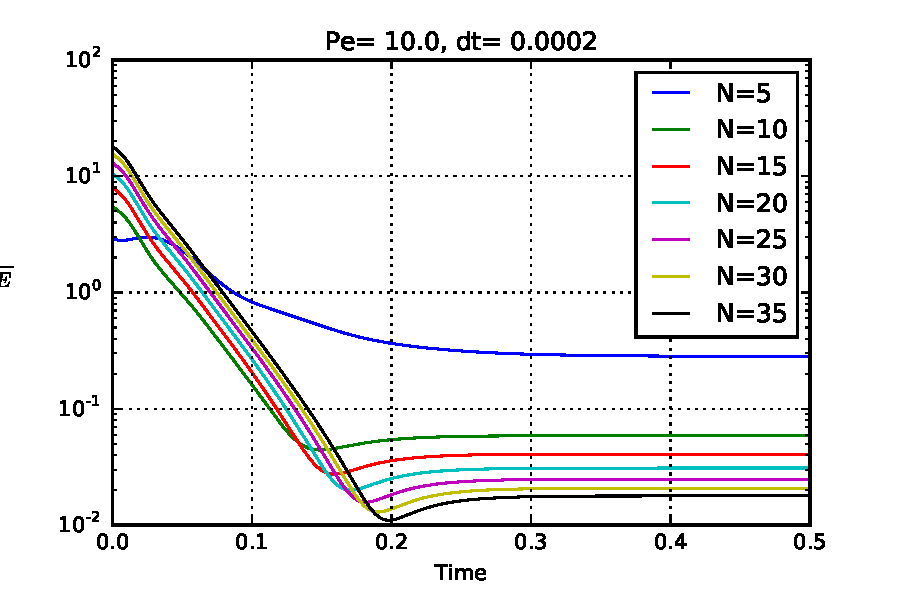
\includegraphics[width=0.8\textwidth]{/home/marszal/Projects/Num_Str_final/FTCS/plots/sse_over_time.pdf}\caption{Sum of squared errors (SSE) der numerischen Integration im Vergleich zu dem Referenzfeld $T^*$.}\label{fig:Performance1}
\end{figure}
\begin{figure}
\centering
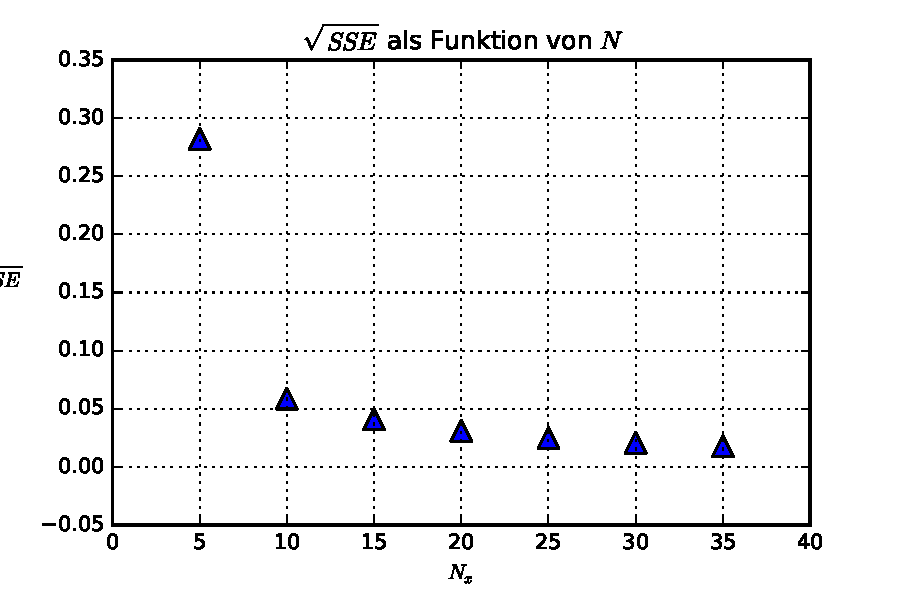
\includegraphics[width=0.8\textwidth]{/home/marszal/Projects/Num_Str_final/FTCS/plots/SSE_at_end.pdf}\caption{Sum of squared errors (SSE) der numerischen Integration im Vergleich zu dem Referenzfeld $T^*$.}\label{fig:Performance1}
\end{figure}
Eine SSE von nur 0.02 ist durchaus akzeptabel, vor allem da dies einer noch geringeren Abweichung der einzelnen Gitterpunkte von $T^*$ entspricht, da die SSE nicht auf die Anzahl der Gitterpunkte normiert ist. Damit lässt sich sagen, dass das FTCS-Verfahren eine physikalisch sinnvolle Lösung des Problems liefert.
\subsection{Vergleich unterschiedlicher Peclet-Zahlen}
Nun da bekannt ist, dass die numerische Lösung des Verfahrens eine korrekte Lösung des Problems liefert, kann das ursprüngliche Problem aus \cref{Gl:PDGL} genauer betrachtet werden.
In \cref{fig:A4} sind die Temperaturfelder für die Peclet-Zahlen $Pe~=2$ und $Pe~=10$ zu den Zeiten $t = 0.005,0.05$ und $0.5$ visualisiert. Die Gittergröße beträgt wieder $N=30$ und die Zeitschrittweite $dt=0.0002$.

Aus dem Vergleich wird deutlich welchen Einfluss die Peclet-Zahl auf die Dynamik des Systems hat. Eine größere Peclet-Zahl führt zu einer schnelleren advektiven Veränderung des Temperaturfeldes.

\begin{figure}
  \centering
    \begin{subfigure}[b]{0.48\textwidth}
      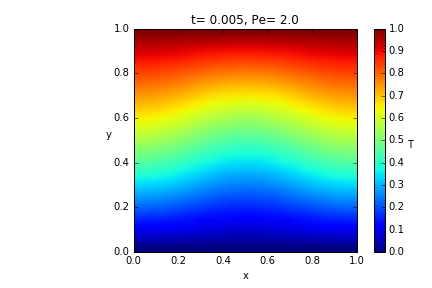
\includegraphics[width=1.15\textwidth]{/home/marszal/Projects/Num_Str_final/FTCS/plots/A4/Pe2/0.005_2_30_30_0.0002_0.txt.png}
    \end{subfigure}
    ~
    \begin{subfigure}[b]{0.48\textwidth}
      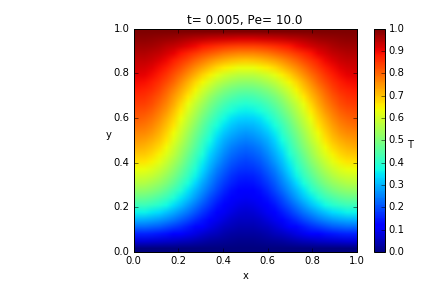
\includegraphics[width=1.15\textwidth]{/home/marszal/Projects/Num_Str_final/FTCS/plots/A4/Pe10/0.005_10_30_30_0.0002_0.txt.png}
    \end{subfigure}
    \\
    \begin{subfigure}[b]{0.48\textwidth}
      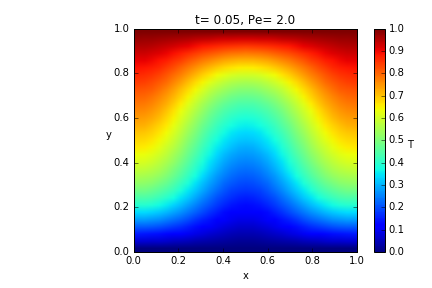
\includegraphics[width=1.15\textwidth]{/home/marszal/Projects/Num_Str_final/FTCS/plots/A4/Pe2/0.05_2_30_30_0.0002_0.txt.png}
    \end{subfigure}
    ~
    \begin{subfigure}[b]{0.48\textwidth}
      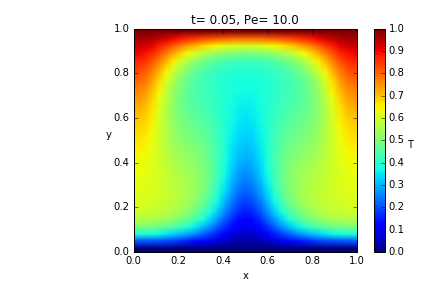
\includegraphics[width=1.15\textwidth]{/home/marszal/Projects/Num_Str_final/FTCS/plots/A4/Pe10/0.05_10_30_30_0.0002_0.txt.png}
    \end{subfigure}
    \\
    \begin{subfigure}[b]{0.48\textwidth}
      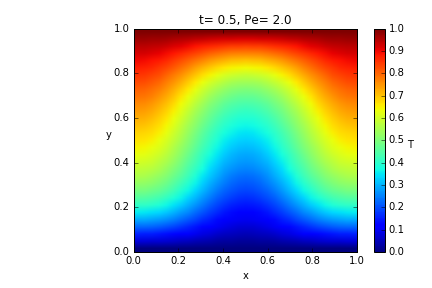
\includegraphics[width=1.15\textwidth]{/home/marszal/Projects/Num_Str_final/FTCS/plots/A4/Pe2/0.5_2_30_30_0.0002_0.txt.png}
    \end{subfigure}
    ~
    \begin{subfigure}[b]{0.48\textwidth}
      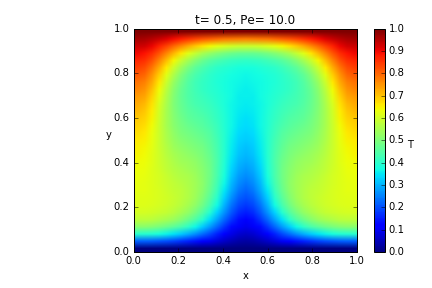
\includegraphics[width=1.15\textwidth]{/home/marszal/Projects/Num_Str_final/FTCS/plots/A4/Pe10/0.5_10_30_30_0.0002_0.txt.png}
    \end{subfigure}
    \\
    \begin{subfigure}[b]{0.48\textwidth}
      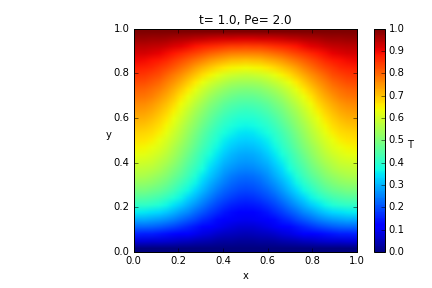
\includegraphics[width=1.15\textwidth]{/home/marszal/Projects/Num_Str_final/FTCS/plots/A4/Pe2/1_2_30_30_0.0002_0.txt.png}
    \end{subfigure}
    ~
    \begin{subfigure}[b]{0.48\textwidth}
      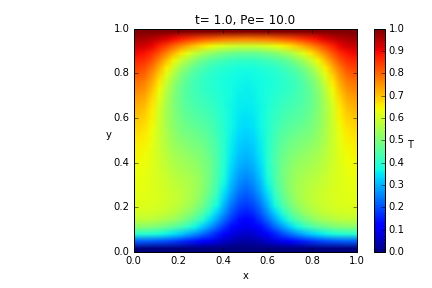
\includegraphics[width=1.15\textwidth]{/home/marszal/Projects/Num_Str_final/FTCS/plots/A4/Pe10/1_10_30_30_0.0002_0.txt.png}
    \end{subfigure}
  \caption{Temperaturfeld zu verschiedenen Zeiten und verschiedenen $Pe$. Berechnet mit dem FTCS-Verfahren. Links $Pe~=2$, rechts $Pe=10$.}\label{fig:FTCSnaive}
\end{figure}
\subsection{Zulässige Zeitschritte}
Bis jetzt wurde immer der Zeitschritt $dt=0.0002$ verwendet. Aus den obigen Simulationen ging eindeutig hervor, dass für die betrachteten Gittergrößen und Peclet-Zahlen dieser Zeitschritt noch ein stabiles Verfahren liefert.
Jetzt wird untersucht ab welcher Größe der Zeitschritt zu einer Divergenz des Verfahrens führt.

Eine theoretische Grenze für die Stabilität des Verfahrens wird durch das CFL-Kriterium für Diffusions- und Advektionsgleichungen vorgegeben.
Für die Stabilität des Diffusionsterms muss folgende Ungleichung gelten:
\begin{align}
  \frac{\Delta t}{\Delta x^2}+\frac{\Delta t}{\Delta y^2} < CFL. \label{eq:CFLdiff}
\end{align}
Wobei die CFL-Zahl für diese Ungleichung als $0.5$ angenommen wird. Intuitiv lässt sich diese Gleichung verstehen als die Bedingung, dass die mittlere quadratische Verschiebung durch die Diffusion in einem Zeitschritt den Abstand zweier Gitterpunkte nicht übersteigen darf. Für eine Diffusionskonstante von $1$ ergibt sich damit die CFL-Zahl $0.5$.

Die zweite Stabilitätsbedingung des FTCS-Verfahrens rührt von dem Advektionsterm her und ist ähnlich zu verstehen wie \cref{eq:CFLdiff}. In einem Zeitschritt darf die Verschiebung der Temperatur nur maximal den nächsten Gitterpunkt erreichen.
Die Ungleichung für den zwei dimensionalen Fall lautet:
\begin{align}
  \frac{Pe~u_{max} \Delta t}{\Delta x} +\frac{Pe~v_{max} \Delta t}{\Delta y}  < CFL = 1. \label{eq:CFLAdv}
\end{align}
Für unser gegebenes Geschwindikeitsfeld ergibt sich $u_{max} = \pi$ und $v_{max} = 2\pi$. In \cref{fig:CFL} sind die Stabilitätsgrenzen als Funktionen der Peclet-Zahl dargestellt. Der Umschlag des jeweils geltenden Kriteriums befindet sich bei $Pe~=12.56$ für eine konstant gehaltene Gittergröße mit $N=30$.
\begin{figure}
  \centering
  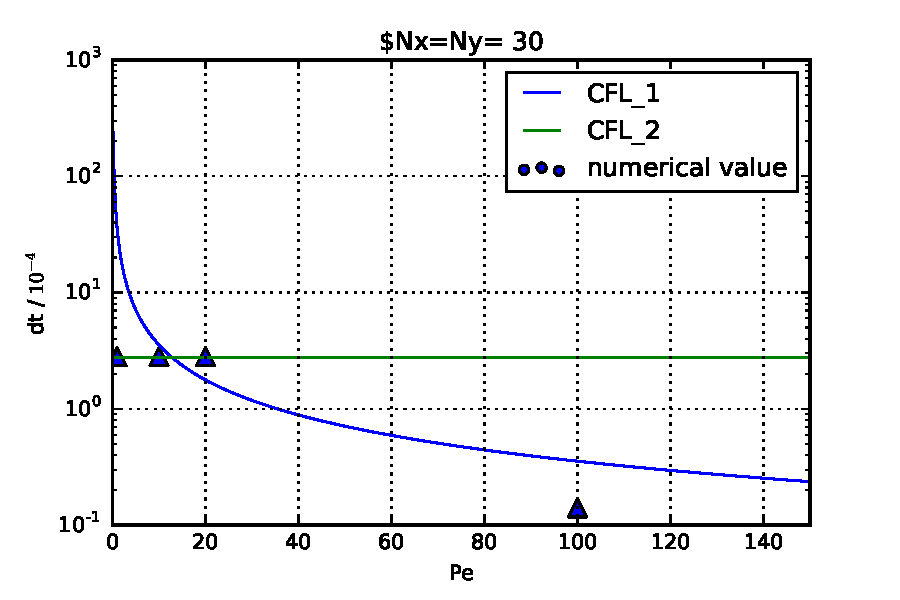
\includegraphics[width=0.7\textwidth]{/home/marszal/Projects/Num_Str_final/FTCS/plots/A5/theoretical.pdf}
  \caption{Theoretisch erwartete Grenzen für die Stabiliät in Abhängigkeit von der Peclet-Zahl. Die Punkte markieren die in \cref{fig:stab} gefundenen maximal stabilen Werte.}\label{fig:CFL}
\end{figure}

Für die Peclet-Zahlen $Pe~=(0.1,1,10,20,100)$ wurde das System mit unterschiedlichen Zeitschritten integriert. \cref{fig:stab} zeigt die Entwicklung des Mittelwertes der Beträge der Gitterpunkte. Die jeweils größten stabilen Zeitschritte sind in \cref{fig:CFL} als Punkte eingetragen.

Aus der Analyse von \cref{fig:stab} geht hervor, dass für $Pe~=(0.1,1,10,20)$ selbst Zeitschritte, die leicht über der Stabilitätsschranke liegen, noch stabil erscheinen.

Allerdings geht aus den Simulationen hervor, dass die der Divergenz für kleinere Zeitschritte später einsetzt, bzw. erkennbar wird. Daraus kann man schließen, dass man bessere Näherungen für den maximalen stabilen Zeitschritt erhält wenn man den Integrationszeitraum erhöht.

Ein anderes Problem tut sich jedoch auf wenn man $Pe~=100$ betrachtet. Diese wurde hier lediglich betrachtet, weil der Umschlag der Stabilitätsgrenze bei $Pe~=20$ nicht erkennbar war, wahrscheinlich wegen des oben beschriebenen Phänomens.

Im Gegensatz zu den kleineren Peclet-Zahlen, liefert die numerische Untersuchung von $Pe~=100$ Zeitschritte die nach \cref{eq:CFLAdv} stabil sein sollten, aber in der Praxis zu Divergenz führen.

Diese Tatsache verdeutlicht, dass es sich bei den CFL-Kriterien nur um notwendige Kriterien handelt und nicht um hinreichende. Eine Neumann'sche Stabilitätsanalyse könnte weitere Kriterien für die Stabilität des Verfahren für größere Peclet-Zahlen aufzeigen.

\begin{figure}
  \centering
  \begin{subfigure}[b]{0.5\textwidth}
  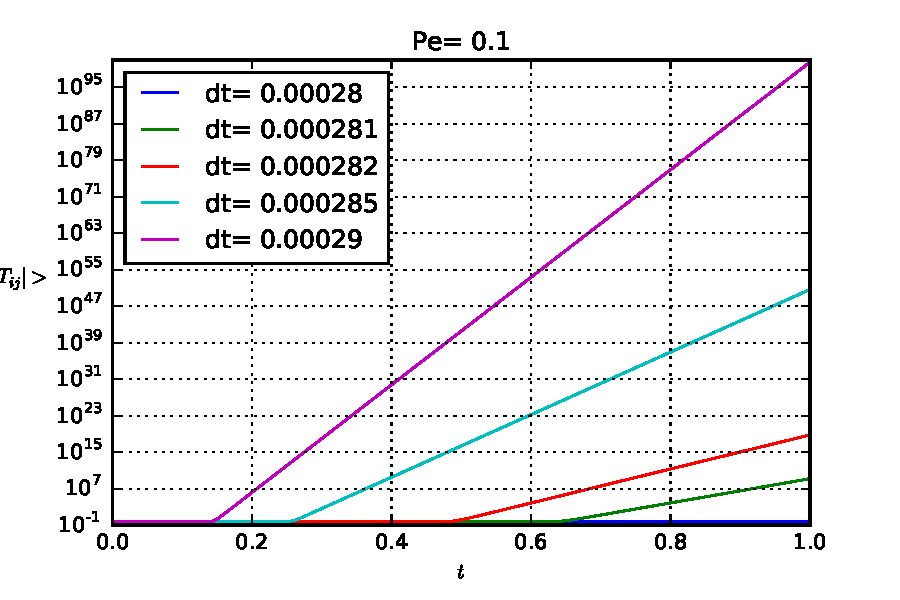
\includegraphics[width=\textwidth]{/home/marszal/Projects/Num_Str_final/FTCS/plots/A5/Divergence_Pe0.1.pdf}
  \end{subfigure}
  \hspace{-0.5cm}
  \centering
  \begin{subfigure}[b]{0.5\textwidth}
  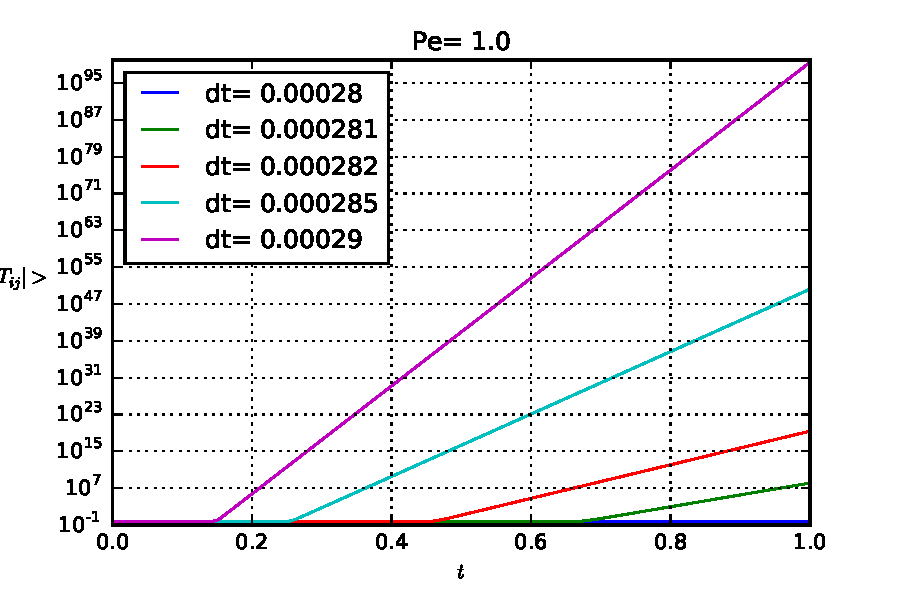
\includegraphics[width=\textwidth]{/home/marszal/Projects/Num_Str_final/FTCS/plots/A5/Divergence_Pe1.0.pdf}
  \end{subfigure}
  \hspace{-0.5cm}
  \centering
  \begin{subfigure}[b]{0.5\textwidth}
  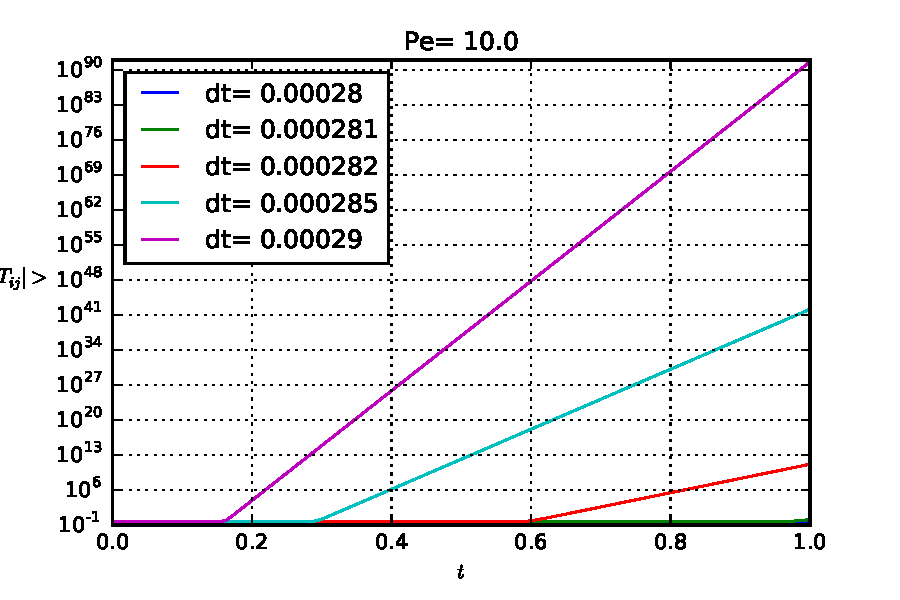
\includegraphics[width=\textwidth]{/home/marszal/Projects/Num_Str_final/FTCS/plots/A5/Divergence_Pe10.0.pdf}
  \end{subfigure}
  \hspace{-0.5cm}
  \centering
  \begin{subfigure}[b]{0.5\textwidth}
  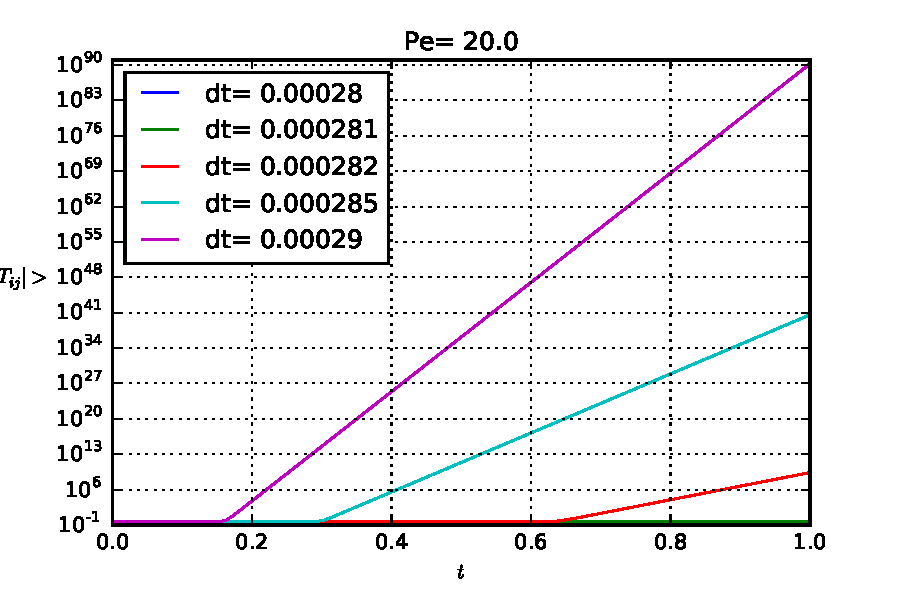
\includegraphics[width=\textwidth]{/home/marszal/Projects/Num_Str_final/FTCS/plots/A5/Divergence_Pe20.0.pdf}
  \end{subfigure}
  \hspace{-0.5cm}
  \centering
  \begin{subfigure}[b]{0.5\textwidth}
  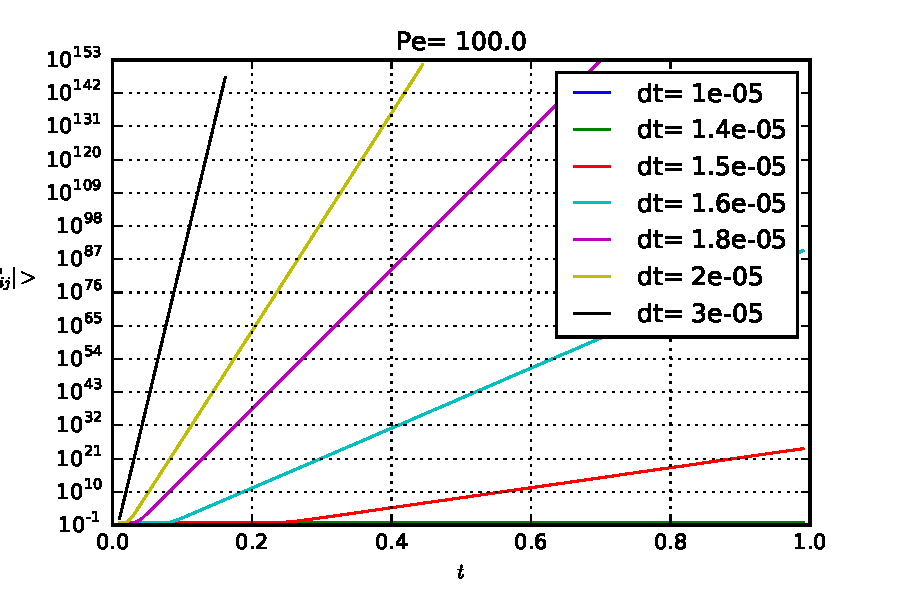
\includegraphics[width=\textwidth]{/home/marszal/Projects/Num_Str_final/FTCS/plots/A5/Divergence_Pe100.0.pdf}
  \end{subfigure}
  \caption{Suche nach dem maximalen stabilen Zeitschritt für verschiedene Peclet-Zahlen.}\label{fig:stab}
\end{figure}
\subsection{Feineinstellung des SOR-Algorithmus}
Da in jedem Zeitschritt des BTCS-Verfahrens ein lineares Gleichungssystem in $N\cdot(N-2)$ Dimensionen gelöst werden muss, und dies Rechenzeit in Anspruch nimmt, ist es sinnvoll das SOR-Verfahren zu optimieren.
Gesucht ist nun der Relaxationsparameter $\omega$, für welchen die geringste Anzahl an Schritten nötig ist um die Gleichung bis auf eine bestimmte Fehlergrenze zu lösen.

Als Testgleichung wird $M\boldsymbol x = \boldsymbol T^0$ verwendet. Wobei $\boldsymbol T^0$ die Anfangsbedingung unseres Problems darstellt.

Ein Parameterscan in $\omega$ wurde für die Matrizen $M$ mit Parametern $Pe~=10$, $dt=100$, $N=30$ und $Pe~=10$, $dt=0.0002$, $N=30$ durchgeführt. Als Fehlergrenze für $|\boldsymbol r_n|$ wird $10^{-4}$ gewählt.
Die Ergebnisse sind in \cref{fig:parscan100} und \cref{fig:parscan000} dargsetellt.

Es zeigt sich dass der optimale Wert für $\omega$ stark von der Matrix $M$ abhängt.
Nicht nur da Minimum der Funktion liegt an unterschiedlichen Positionen ($\omega_{min}=1.599$ für $\Delta t=100$ und $\omega_{min}=1.1$ für $\Delta t=0.0002$), auch das Profil der Iterationen für jedes $\omega$ verändert sich stark. Für \cref{fig:parscan100} explodiert die Anzahl der benötigten Iterationen kurz nach erreichen des optimalen Relaxationsparameters, während das Minimum bei einem Zeitschritt von $dt=0.0002$ wesentlich flacher ist.

Daraus lässt sich schließen, dass die Genauigkeit der Wahl des Relaxationsparameters bei bestimmten Matrizen einen bedeutenden Einfluss auf die Geschwindigkeit des Algorithmus nehmen kann.

\begin{figure}
\centering
\begin{subfigure}[b]{0.45\textwidth}
  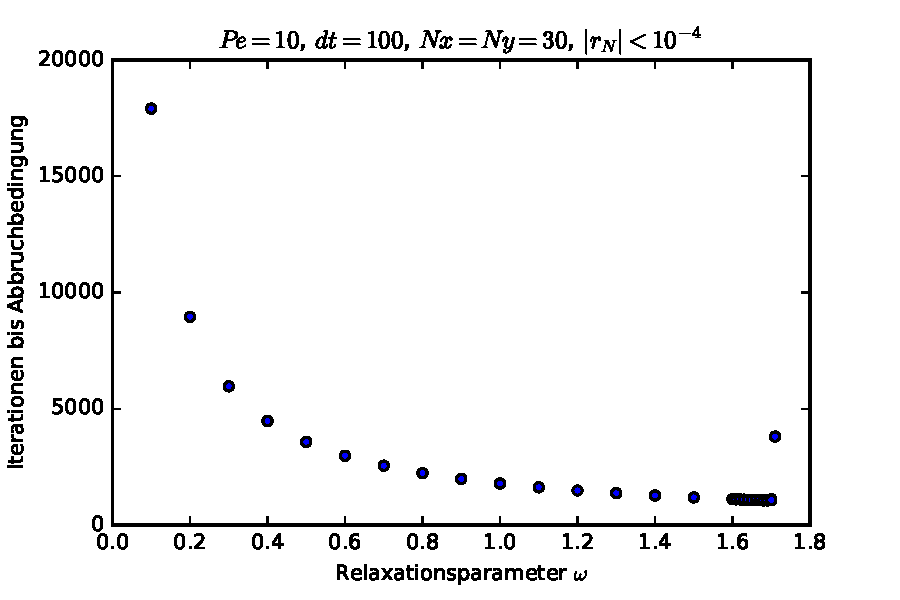
\includegraphics[width=\textwidth]{/home/marszal/Projects/Num_Str_final/BTCS/plots/omegascan_dt100.pdf}\caption{Parameterscan in $\omega$ für die Parameter $Pe~=10$, $dt=100$ und $N=30$. Der optimale $\omega$-Wert liegt bei etwa 1.599.}\label{fig:parscan100}
\end{subfigure}
~
\begin{subfigure}[b]{0.45\textwidth}
  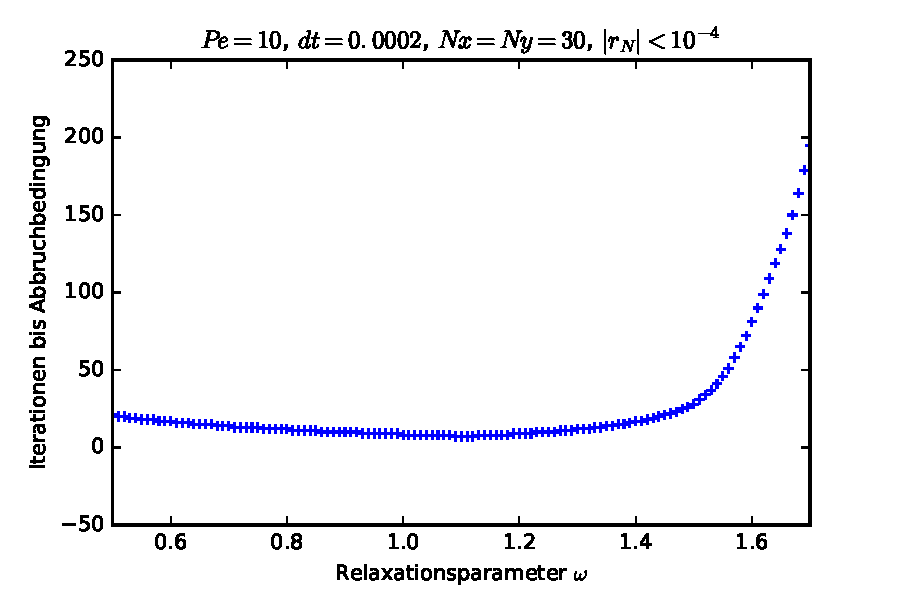
\includegraphics[width=\textwidth]{/home/marszal/Projects/Num_Str_final/BTCS/plots/omegascan_dt0.0002.pdf}\caption{Parameterscan in $\omega$ für die Parameter $Pe~=10$, $dt=0.0002$ und $N=30$. Der optimale $\omega$-Wert liegt bei etwa 1.1.}\label{fig:parscan000}
\end{subfigure}
\end{figure}

\subsection{Vergleich FTCS und BTCS}
Mit dem optmimierten SOR-Verfahren kann nun sinnvoll ein Vergleich zwischen dem FTCS- und dem BTCS-Verfahren durchgeführt werden.
Für die Parameter $Pe~=10$, $dt=0.0002$ und $N=30$ is in \cref{fig:vergleich} das Temperaturfeld für verschieden Zeitpunkte, mit dem FTCS- und dem BTCS-Verfahren integriert, aufgezeigt.

Es sind keine starken Unterschiede zu erkennen. Man kann unter Umständen eine Abweichung zur Zeit $t=0.0054$ erkennen, diese ist aber nur sehr schwach ausgeprägt.

\begin{figure}
  \centering
  \begin{subfigure}[b]{0.5\textwidth}\caption{BTCS}
  \includegraphics[width=\textwidth]{/home/marszal/Projects/Num_Str_final/BTCS/plots/0.0054_10_30_30_0.0002_0.txt.png}
  \end{subfigure}
  \hspace{-0.5cm}
  \begin{subfigure}[b]{0.5\textwidth}\caption{FTCS}
  \includegraphics[width=\textwidth]{/home/marszal/Projects/Num_Str_final/FTCS/plots/compare/0.0054_10_30_30_0.0002_0.txt.png}
  \end{subfigure}
  \\
  \begin{subfigure}[b]{0.5\textwidth}
  \includegraphics[width=\textwidth]{/home/marszal/Projects/Num_Str_final/BTCS/plots/0.0508_10_30_30_0.0002_0.txt.png}
  \end{subfigure}
  \hspace{-0.5cm}
  \begin{subfigure}[b]{0.5\textwidth}
  \includegraphics[width=\textwidth]{/home/marszal/Projects/Num_Str_final/FTCS/plots/compare/0.0508_10_30_30_0.0002_0.txt.png}
  \end{subfigure}
  \\
  \begin{subfigure}[b]{0.5\textwidth}
  \includegraphics[width=\textwidth]{/home/marszal/Projects/Num_Str_final/BTCS/plots/0.5002_10_30_30_0.0002_0.txt.png}
  \end{subfigure}
  \hspace{-0.5cm}
  \begin{subfigure}[b]{0.5\textwidth}
  \includegraphics[width=\textwidth]{/home/marszal/Projects/Num_Str_final/FTCS/plots/compare/0.5002_10_30_30_0.0002_0.txt.png}
  \end{subfigure}
  \caption{Vergleich zwischen den Temperaturfeldern, wie sie durch die BTCS- und FTCS-Integration zustande kommen.}\label{fig:vergleich}
\end{figure}

Einen deutlicheren Unterschied bildet die Laufzeit der beiden Verfahren. Kleine Integrationszeiträume von $t_{end}=0.5$ werden vom FTCS-Verfahren mit dem maximal möglichen Zeitschritt von 0.000277 in weniger als $1$~s gelöst. Das BTCS-Verfahren benötigt dafür mit einem Zeitschritt von 0.5 ca. 55~s.

Bei längeren Integrationszeiträumen jedoch stößt die FTCS-Methode an ihre Grenzen, da sie nur für sehr kleine Zeitschritte stabil ist.
Dadurch werden wesentlich mehr Iterationen benötigt, wodurch die Laufzeit anwächst.
Die BTCS-Methode kann selbst bei großen Zeitschritten ein gutes Ergebnis liefern, wie in \cref{fig:vergleich2} zu sehen ist.

Für einem Integrationzeitraum von $t_{end}=100$ liefert das FTCS-Verfahren eine Laufzeit von 120~s und das BTCS-Verfahren eine Laufzeit von 93~s, bei einem Zeitschritt von $\Delta t = 100$.
Damit bestätigt sich die Vermutung, dass implizite Verfahren bei größeren Integrationszeiträumen, und wenn keine hohe Zeitauflösung benötigt wird, die effizientere Alternative zu den expliziten Methoden bilden.

\begin{figure}
\centering
  \begin{subfigure}[b]{0.5\textwidth}\caption{FTCS}
    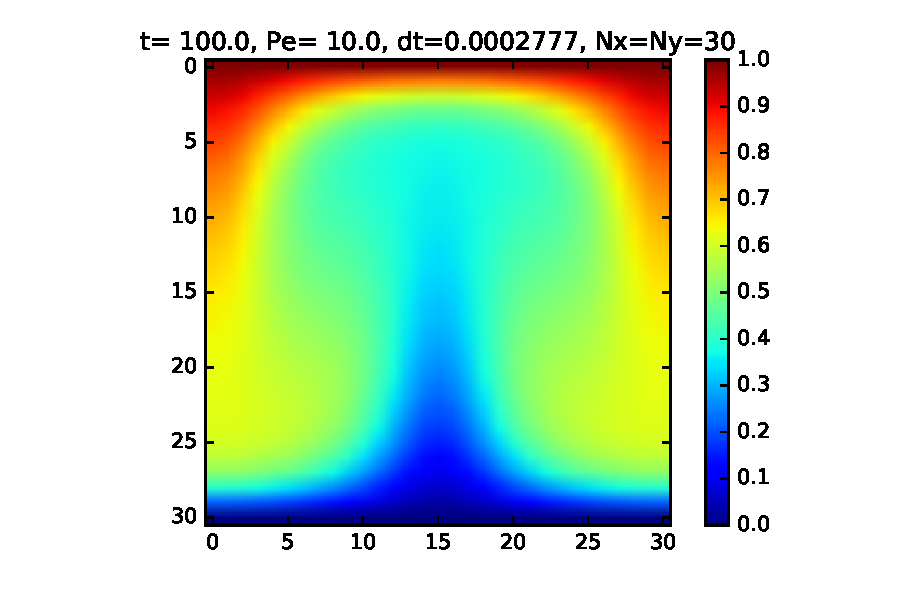
\includegraphics[width=\textwidth]{/home/marszal/Projects/Num_Str_final/BTCS/plots/compare/FTCS100_10_30_30_0.0002777_0.txt.pdf}
  \end{subfigure}
  \hspace{-0.5cm}
  \begin{subfigure}[b]{0.5\textwidth}\caption{BTCS}
    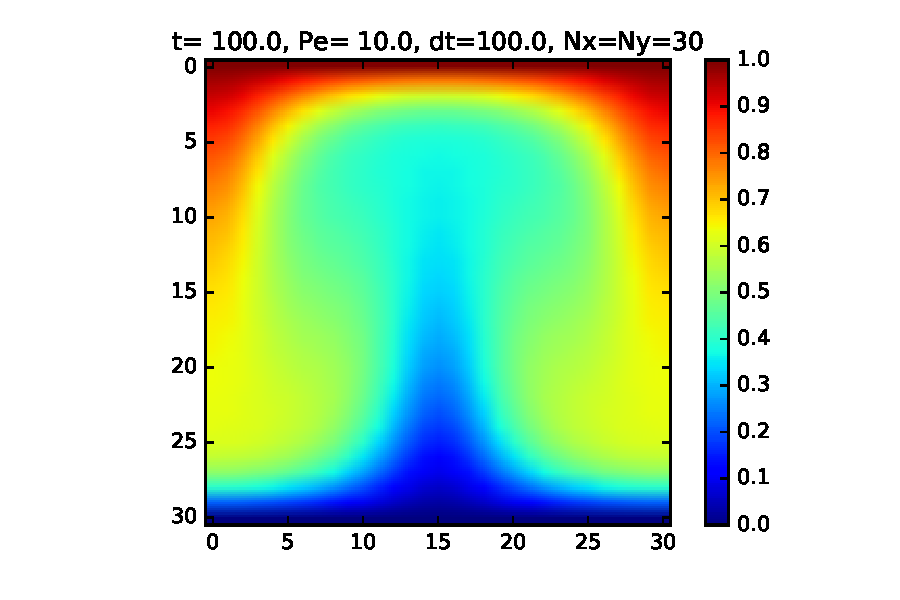
\includegraphics[width=\textwidth]{/home/marszal/Projects/Num_Str_final/BTCS/plots/compare/BTCS100_10_30_30_100_0.txt.pdf}
  \end{subfigure}
  \caption{Vergleich zwischen den Temperaturfeldern, wie sie durch die BTCS- und FTCS-Integration zustande kommen, nach einem Zeitraum von $t=100$.}\label{fig:vergleich2}
\end{figure}
\newpage
\section{Fazit}
Die Vor- und Nachteile der BTCS-und FTCS-Verfahren wurden im Zuge dieser Ausarbeitung deutlich aufgezeigt.
Während das FTCS-Verfahren sehr einfach zu implementieren ist, und pro Zeitschritt sehr effizient rechnet, sind die Möglichkeiten des FTCS-Verfahrens beschränkt. Eine obere Schranke an den Zeitschritt, um die Stabilität des Verfahrens zu garantieren, führt zu überaus langen Laufzeiten für Simulationen großer Zeiträume.

Interessiert man sich für die Simulation langer Zeiträume, bei relativ grober Gittereinteilung, so greift man besser zu dem BTCS-Schema.
Zwar büßt man an Zeitauflösung ein, da man die Anzahl der Zeitschritte möglichst gering halten möchte, gewinnt aber an Stabilität, und ab einer bestimmten Größe des simulierten Zeitraums spart man ebenfalls Laufzeit gegenüber des FTCS-Schemas.

Implementiert man das BTCS-Verfahren, so muss der Relaxationsparameter sorgfältig gewählt werden, da er die Anzahl der Iterationen pro Zeitschritt deutlich reduzieren kann.

\end{document}
